\documentclass[
a4paper,   
headsepline, 
fleqn,     
12pt
]{scrartcl}

%%% ngerman: language set to new-german
\usepackage{ngerman}
\usepackage[latin1]{inputenc}
\usepackage[T1]{fontenc}
\usepackage{ae,aecompl}

%%% Graphic stuff
\usepackage{graphicx}
\usepackage{amsmath,amssymb,amstext}
\usepackage{units}
\usepackage{scrpage2}

\setlength{\parindent}{0em} 

\newcommand{\mygraphics}[3]{
  \begin{center}
    \includegraphics[width=#1, keepaspectratio=true]{#2} \\
    \textbf{#3}
  \end{center}
}

%%%      footer - middle: page number
\pagestyle{scrheadings}

%%% heading - left
 \ihead[]{Marco Sohm, Kevin Wallis}

%%% heading - right
 \ohead[]{Aufgabe 1}

\begin{document}

 \pagenumbering{roman} %% small roman page numbers
 \pagenumbering{arabic} 

\subsection*{Erweiterung des Vorlesungsbeispiels}
Das Vorlesungsbeispiel wurde nach den angegebenen Vorgaben erweitert. Das erweiterte Beispiel ist als Anhang beigef�gt.

\subsection*{Berechnen des Gleichgewichtszustands}
Im Folgenden werden die beiden Gleichungen f�r $\frac{dC_1}{dt}$ und $\frac{dC_2}{dt}$ angegeben.

\begin{itemize}
\item $\frac{0.34*1e6 * 320}{50*1e6} + \frac{C_2 * 0.5*1e6}{50*1e6} - \frac{0.34*1e6 * C_1}{50*1e6}-0.02 * C_1- \frac{0.5*1e6 * C_1}{50*1e6} = 0$
\item $\frac{0.5*1e6 * C_1}{100*1e6}-0.002 * C_2- \frac{0.5*1e6 * C_2}{100*1e6} = 0$
\end{itemize}

Aus der zweiten Gleichung kann $C_2$ wie folgt berechnet werden: $C_2 = 5 * \frac{C_1}{7}$. Dieses Resultat wird in die erste Gleichung eingesetzt. Dadurch ergibt sich die folgende Gleichung:
$\frac{0.34*1e6 * 320}{50*1e6} + \frac{5 * C_1 * 0.5*1e6}{7 * 50*1e6} - \frac{0.34*1e6 * C_1}{50*1e6}-0.02 * C_1- \frac{0.5*1e6 * C_1}{50*1e6} = 0$
Das Umstellen dieser Gleichung ergibt $C_1=73.372$. Dieser Ergebnis wird wiederum in das zuvor berechnete $C_2$ eingesetzt, somit ist $C_2=52.409$. Diese Werte wurden mithilfe der Simulation �berpr�ft (Siehe \ref{fig:Gleichgewicht}).\\

\begin{figure}[h]
  \centering
  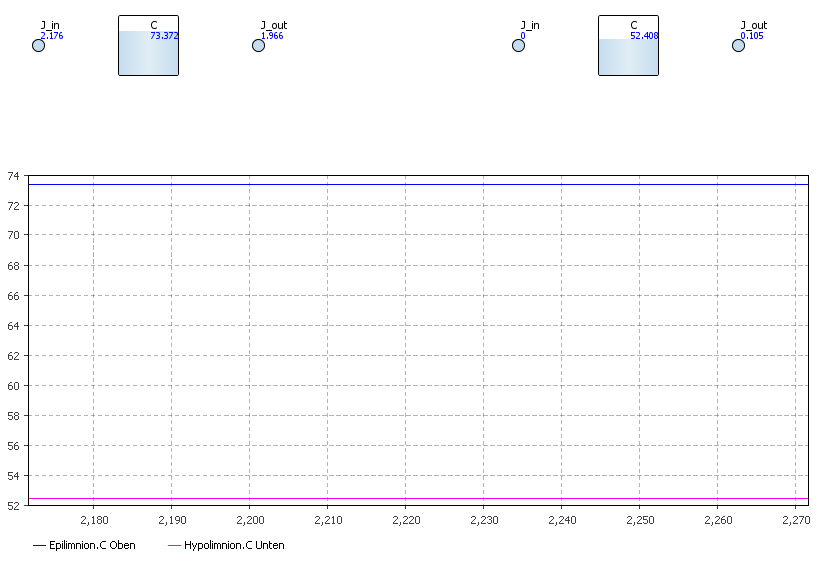
\includegraphics[width=1\textwidth]{./images/Gleichgewicht}
  \caption[Gleichgewicht: Simulation]{Simulation des Gleichgewichts}
  \label{fig:Gleichgewicht}
\end{figure}

Ist das Gleichgewicht stabil? Ja, da das Gleichgewicht bei diesem Beispiel ein Attraktor ist.
Berechnung n�tig?????

\subsection*{Zwischenschichtenmodel f�r den Winter}
Was kann man bez�glich des Gleichgewichts im Vergleich zum vorherigen Zwischenschichtenmodel sagen?
Berechnen des Gleichgewichts
Ist das Gleichgewicht stabil?

\appendix  
\bibliographystyle{plain}
\bibliography{projekt.bib}

\end{document}